\documentclass [11pt, a4wide, twoside]{article}

\usepackage{times}
\usepackage{epsfig}
\usepackage{ifthen}
\usepackage{xspace}
\usepackage{fancyhdr}
\usepackage{moreverb}

% solution switch
\newboolean{showsolution}
\setboolean{showsolution}{true}
\setboolean{showsolution}{false}



%layout
\topmargin      -5.0mm
\oddsidemargin  6.0mm
\evensidemargin -6.0mm
\textheight 215.5mm
\textwidth      160.0mm
\parindent        1.0em
\headsep          10.3mm
\headheight        12pt
\lineskip    1pt
\normallineskip     1pt

%header
\lhead{Programming Languages \\ 2021}

\rhead{Prof. O. Nierstrasz\\
Mohammadreza Hazhirpasand, Joel Niklaus}
\lfoot{page \thepage}
\rfoot{\today}
\cfoot{}

\renewcommand{\headrulewidth}{0.1pt}
\renewcommand{\footrulewidth}{0.1pt}

\renewcommand{\thesubsection}{\arabic{subsection}}

%enumeration
\newenvironment{myitemize}{%
     \begin{itemize}
     \setlength{\itemsep}{0cm}}
     {\end{itemize}}

\newenvironment{myenumerate}{%
     \begin{enumerate} \setlength{\itemsep}{0cm}}
     {\end{enumerate}}


%solution
\ifthenelse{\boolean{showsolution}}
   {  \newcommand{\solution}[1]{
   	\noindent\underline{\textbf{Answer:}}\\[2mm]
   	 \textsl{#1}
	 \vspace{10pt}
	 \normalsize
	}
  }
  {  \newcommand{\solution}[1]{} }

\newcounter{exnum}
\def\xexercise{\fontsize{12}{10}\fontseries{bx}\selectfont}
\def\xnormal{\fontseries{m}\fontshape{n}\selectfont}


\newcommand{\exercise}[1]{%
     {\addtocounter{exnum}{1}\vskip 0.8cm{\xexercise \noindent Exercise
\arabic{exnum} (#1)} \xnormal} \vskip 0.3cm} 
 \newcommand{\aufgabe}[1]{
     {\addtocounter{exnum}{1}\vskip 0.8cm{\xexercise \noindent Aufgabe
\arabic{exnum} (#1)} \xnormal} \vskip 0.3cm} 

\pagestyle{fancy}


% ===============ABBREVIATIONS==============================
\newcommand{\eg}{\emph{e.g.,}\xspace}
\newcommand{\ie}{\emph{i.e.,}\xspace}
\newcommand{\etc}{\emph{etc.}\xspace}


\begin{document}

% title
\section*{\ifthenelse{\boolean{showsolution}}{Solution }{}\xspace{}Serie 11 - Applications of Logic Programming}

% - - - - - - - - - - - - - - - - - - - - - - - - - - - - - - - - - - - - - - - - - - - - - - - - - - - - - - - - - - - - - - - - - - -

\subsection*{Exercise 1: General questions}

\begin{enumerate}
\renewcommand{\theenumi}{\alph{enumi}}

\item What are definite clause grammars (DCG) and why are they particularly useful in conjunction with Prolog?
\solution{Definite clause grammars are an extension of context-free grammars. One can easily implement a concrete grammar (e.g. expressed in BNF) by means of a DCG, and the corresponding syntactic rules are directly implementable as Prolog rules. DCG rules in Prolog are just syntactic sugar for ordinary Prolog rules.}

\item How are DCG specifications translated into Prolog?
\solution{In most Prolog versions, it is a DCG interpreter which translates DCG rules into Prolog. The interpreter reads them in the form $Head\to Body$. $Head$ is always a non-terminal, and $Body$ is a sequence of terminals and non-terminals.}

\item What exactly does the 'C' predicate do? And what would be a possible explanation for its rather not meaningful name?
\solution{The 'C' predicate is used to translate (recognize) terminal symbols. It takes a symbol from the input list, and outputs also the remainder of the list for further examination. Essentially, it's a procedure for consuming tokens. It could be defined as follows:\\[2mm]
\texttt{ 'C'([Sym|Tail],Sym,Tail).}\\[2mm]
This predicate is normally not applied by the programmer, but by Prolog's DCG interpreter. This explains its obscure name.}

\item Why are left-associative grammar rules problematic?
\solution{Prolog code shouldn't have left-recursive clauses, otherwise one risks to produce infinite loops. Remember: resolution is always applied from left to right.}
	
\item How can we represent syntax trees in Prolog?
\solution{We can represent syntax trees in Prolog as functions. A node with $n$ children is a function with $n$ arguments, one argument per child. A leaf is a value.}

\item Why must DCG side conditions be put in curly brackets \{\}?
\solution{Curly brackets are solely used for side conditions in DCG. Since the side conditions are pure Prolog and thus should not be translated into Prolog, we need a way to tell the DCG interpreter that it is pure Prolog code. And since the interpreter cannot easily find out itself where a side condition starts and ends, the brackets are a useful means to make it clear.}

\end{enumerate}


%----------------------------------------------------------------------------------------------------
\subsection*{Exercise 2: Hanoi Towers}
The objective of this famous puzzle is to move $N$ disks from the left peg to the right peg using the center peg as an auxiliary holding peg. It is not allowed to place a larger disk on a smaller disk, and only one disk can be taken away at once from the top. The following diagram depicts the starting setup for $N=3$ disks:
%
\begin{figure}[htb]
    \centering{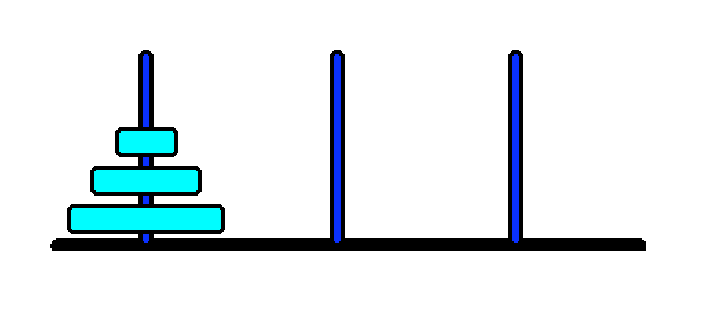
\includegraphics[width=5cm, height=3cm]{hanoi.pdf}}
\end{figure}
%
\noindent Define a predicate \texttt{hanoi(N, A, B, C, Moves)} that solves the hanoi-towers problem. \texttt{Moves} holds the list of moves that represent the process of moving \texttt{N} disks from \texttt{A} to \texttt{B} with the help of \texttt{C}. If \texttt{N} is bigger than 1, then \texttt{N-1} disks will be shifted to \texttt{C}, so that the move from \texttt{A} to \texttt{B} can be accomplished. The move of a disk from \texttt{A} to \texttt{B} will be represented as \texttt{[a to b]}. The binary operator \emph{to} is loaded into the knowledge base by the following commands:
\begin{verbatim}
  :- ensure_loaded(library(operators)). % load readable operators
  :- op(900, xfy, to).                  % define new infix operator 'to'
\end{verbatim}
\noindent Examples:
\begin{verbatim}
  ?- hanoi(1,a,b,c,X).		
  X = [a to b] ?			
  yes					

  ?- hanoi(2,a,b,c,X).
  X = [a to c, a to b, c to b] ?
  yes
\end{verbatim}

\solution{\fontsize{8}{10}\verbatimtabinput{ex2.tex}}


% - - - - - - - - - - - - - - - - - - - - - - - - - - - - - - - - - - - - - - - - - - - - - - - - - - - - - - - - - - - - - - - - - - -

\end{document}
